\documentclass[tikz,border=5pt]{standalone}
\usepackage{pgfplots}
\usetikzlibrary{arrows.meta}
\pgfplotsset{compat=1.18}

\definecolor{corba}{HTML}{365FB3}
\definecolor{assimptota}{HTML}{C2415D}

\begin{document}
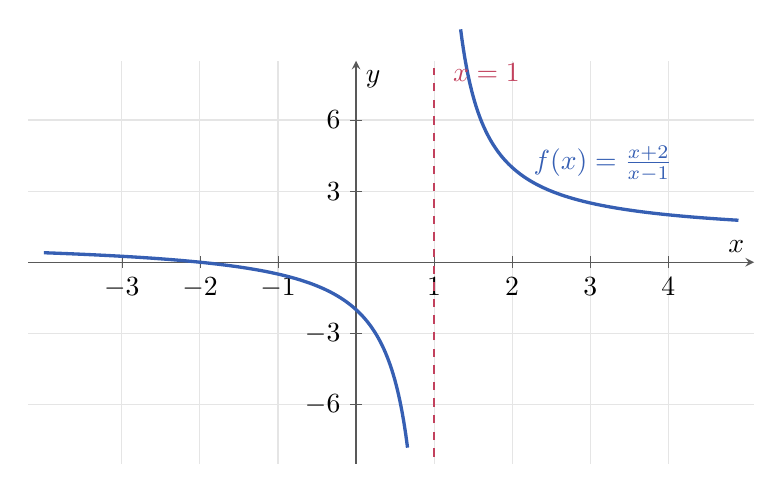
\begin{tikzpicture}
  \begin{axis}[
    width=10.8cm,
    height=6.7cm,
    axis lines=middle,
    xmin=-4.2,
    xmax=5.1,
    ymin=-8.5,
    ymax=8.5,
    xlabel={$x$},
    ylabel={$y$},
    xtick={-3,-2,-1,1,2,3,4},
    ytick={-6,-3,3,6},
    axis line style={black!65},
    tick style={black!65},
    grid=major,
    grid style={black!10},
    clip=false,
  ]
    \addplot[assimptota, dashed, thick] coordinates {(1,-8.2) (1,8.2)};
    \addplot[corba, very thick, domain=-4:0.66, samples=200]
      {(x+2)/(x-1)};
    \addplot[corba, very thick, domain=1.34:4.9, samples=200]
      {(x+2)/(x-1)};

    \node[anchor=south west, text=assimptota]
      at (axis cs:1.12,7.2) {$x=1$};
    \node[anchor=south west, text=corba]
      at (axis cs:2.15,3.0) {$f(x)=\frac{x+2}{x-1}$};
  \end{axis}
\end{tikzpicture}
\end{document}
